\documentclass[7pt,a4paper]{article}

\usepackage{graphicx}
\usepackage{sectsty}

\sectionfont{\fontsize{10}{11}\selectfont}
\subsectionfont{\fontsize{10}{11}\selectfont}

\begin{document}
\textbf{\LARGE Assignment 2c Report - Text Mining}
\section{Introduction}
Given a collection of text documents we aim to find similar documents. In order to do that we normalized the text and created a Tf-idf matrix and perform LSA using reduced latent space with 4 dimensions. For each topic we identify the set of 5 top weighted terms. Find the similarity matrix for the documents in the reduced space. Apply hierarchical clustering. Cut the dendrogram at k and identify clusters of similar documents.

\section{Packages Used - \textit{(Language: Python)}}
\begin{itemize}
\item{\textbf{Sklearn}:Package used for constructing Tf-idf, LSA, cosine similarity.}
\item{\textbf{NLTK}: Package used for Natural Language Processing.}
\item{\textbf{Scipy}: Package which provides function for plotting dendogram and linkage for Hierarchical Clustering.}
\item{\textbf{Seaborn}: Used for visualization of data through plots}
\item{\textbf{Matplotlib}: Used for plotting of graphs}
\item{\textbf{Pandas}: Package which provides Data structure like DataFrame which makes
manipulation of datasets easy}
\end{itemize}

\section{Dataset}
Twenty two text documents were taken all being on the Topic- \textbf{‘The History of web search engines’}. Texts are preprocessed and consists of terms corresponding to each document. 

\section{Methods and Observations}
\subsection{Tf-idf}
Stands for term frequency and inverse document frequency, is a numerical statistic that is intended to reflect how important a word is to a document in a collection.
Formula: tf-idf : tf * idf 
 				 

\subsection{Cosine similarity}
\begin{itemize}
\item{It normalizes the lengths of the documents so smaller documents and longer documents have weights of the same order of magnitude.}
\item{According to the similarity matrix as shown in the figure, most similar documents comes out to be \textit{Ass1-422} and \textit{Ass1-440} (Similarity - 0.57) while the most dissimilar documents are \textit{Ass1-202} and \textit{Ass1-1046} (Similarity - 0.025)}
\textbf{Comparison with the previous Similarity matrix using Jaccard coefficient}
\begin{itemize}
\item{J.C. does not consider the frequencies of the terms in order to calculate the similarity between documents where as cosine similartity has been calculated using tf-idf vectors of the documents so the similarity between documents has increased as the term frequencies has been taken into account}
\end{itemize}
\end{itemize}
\begin{figure}[h]
\centering
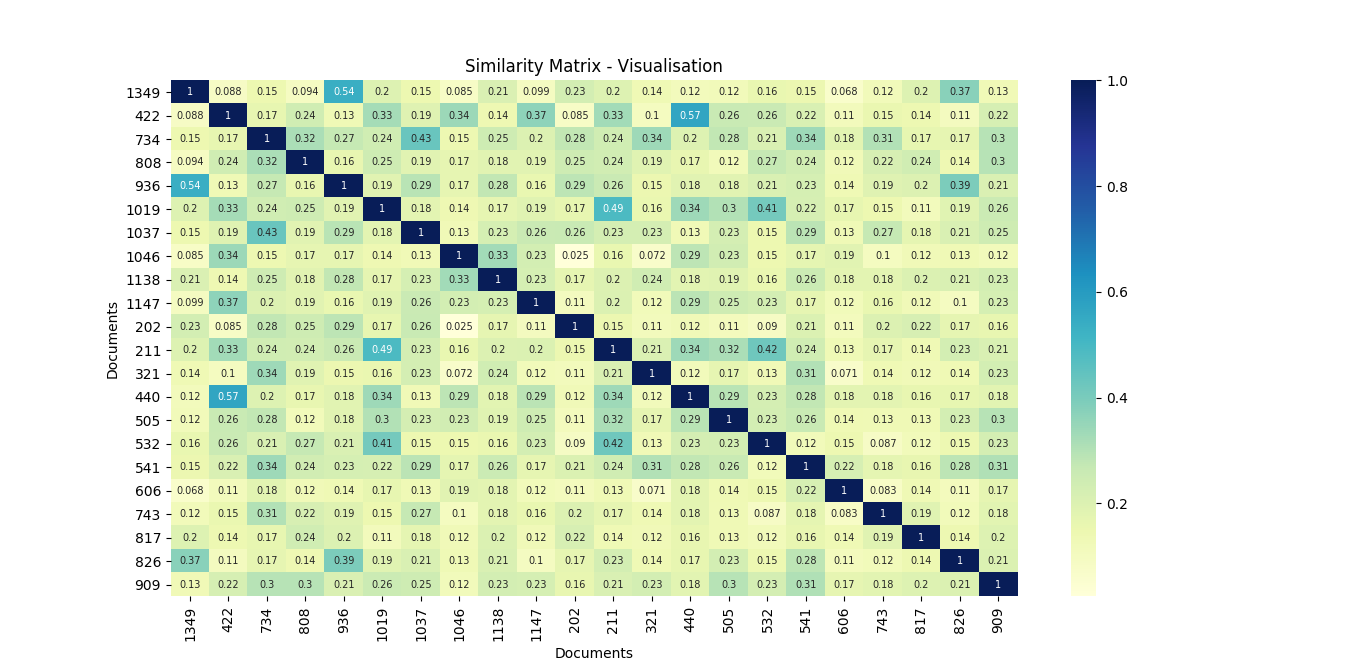
\includegraphics[scale=.40]{sim}
\caption{Similarity matrix - Cosine Similarity}
\label{image-Cos}
\end{figure}

\subsection{Hierarchical Clustering}
\begin{itemize}
\item{\textbf{Distance matrix}: It is obtained by calculating \textit{(1-Cosine Similarity)} between each pair of the documents as shown in the figure}
\item{\textbf{Linkage Parameter} : Single Linkage}
\item{Dendogram is shown in the figure \ref{image-Dendogram} below where the horizontal axis represents the pairwise dissimilarity between documents}

\begin{figure}[h]
\centering
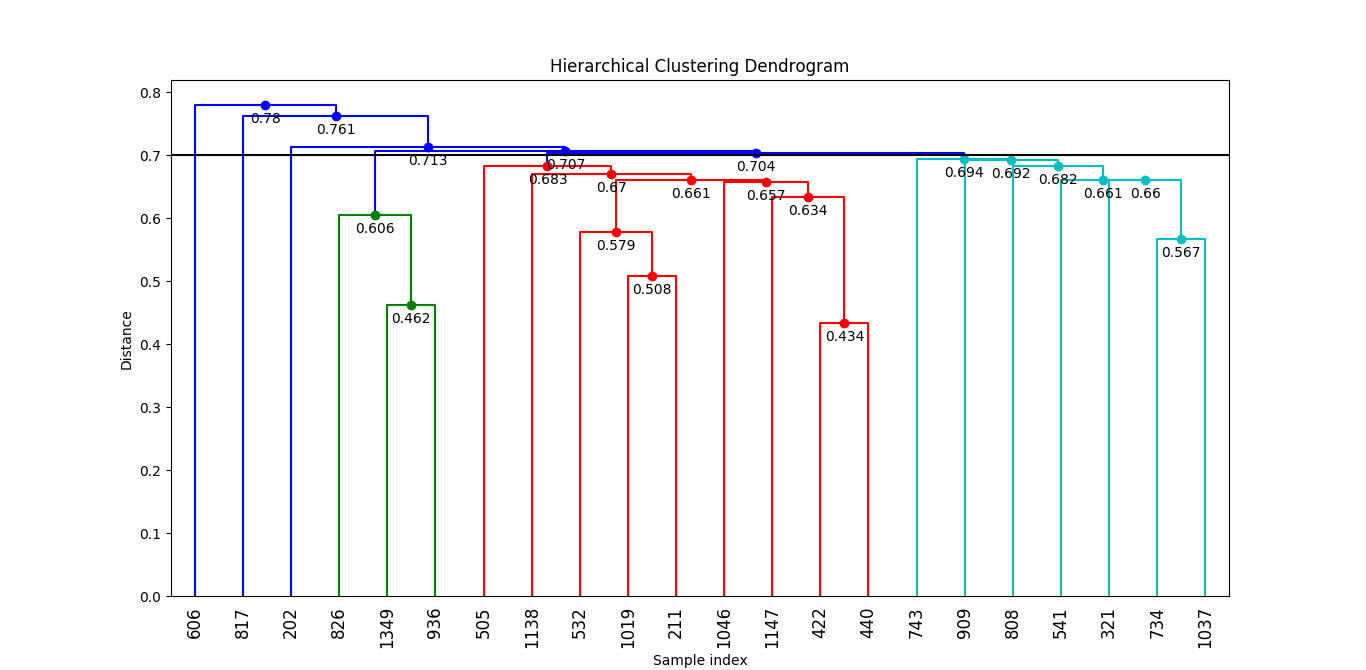
\includegraphics[scale=.40]{dendro}
\caption{Dendrogram}
\label{image-Dendogram}
\end{figure}


\end{itemize}


\end{document}
